\section{Analiza i wizualizacja danych}
Uruchomienie wszystkich scenariuszy symulacji spowodowało wygenerowanie dużej ilości danych (~300GB) rozłożonej na tysiące plików. W celu analizy takiej ilości danych napisany został skrypt w języku Ruby, którego zadaniem była decymacja oraz fuzja wszystkich plików.

Do analizy oraz wizualizacji danych wykorzystany został język R wraz z pakietem ggplot2.

Poniższe wykresy przedstawiają liczbę aktywnych węzłów sieci w czasie oraz w zależności od rozmiaru pakietu i odstępie czasu pomiędzy kolejnymi pakietami. Sieć składała się z dwudziestu węzłów, które rozmieszczone zostały zgodnie z rozkładem normalnym.
Przy rozmiarach pakietu wynoszących 50B i 500B najdłuższy czas działania sieci osiągnięto wykorzystując protokół ALEACH. Czas działania sieci używających wariantów protokołu LEACH uległ wyraźnemu skróceniu przy rozmiarze pakietu wynoszącym 5000B. Wpływ okres pomiędzy pakietami na protokoły typu LEACH jest również zauważalny, jednakże jest on zdecydowanie mniej wyrazisty. Czas działania sieci dla protokołów Flood i SPIN pozostaje niezmienny, niezależnie od dobranych parametrów wykresu. Dodatkowo w ich przypadku dezaktywacja węzłów sieci przebiega gwałtownie oraz lawinowo - większość węzłów sieci zostaje wyłączonych w okolicach jednego punktu w czasie.

Przy rozmiarze pakietu 5B najlepszymi protokołami z punktu widzenia całkowitej długości życia sieci okazały się ALEACH oraz LEACH DCHS.

Przy rozmiarze pakietu 50B najlepszym protokołem z punktu widzenia całkowitej długości życia sieci okazał się ALEACH. W przypadku okresu między pakietami wynoszącym 20s zapewnił on około 50s dłuży czas działania sieci, jednakże protokoły LEACH oraz LEACH DCHS zapewniły dłuży okres jej stabilnego działania.

Przy rozmiarze pakietu 500B wśród protokołów umożliwiających najdłuższe działanie sieci znajduje się ALEACH. Przy okresie 10s LEACH działa lepiej od LEACH DCSH, a w przy okresie 5s i 20s LEACH DCSH działa dłużej niż LEACH.

\clearpage
\thispagestyle{empty}

 {\pdfpagewidth=2\pdfpagewidth
    \vspace*{-2cm}
    \noindent\kern.5\pdfpagewidth\rlap{\parbox{\textwidth}{%
    \noindent\kern.25\pdfpagewidth
        \llap{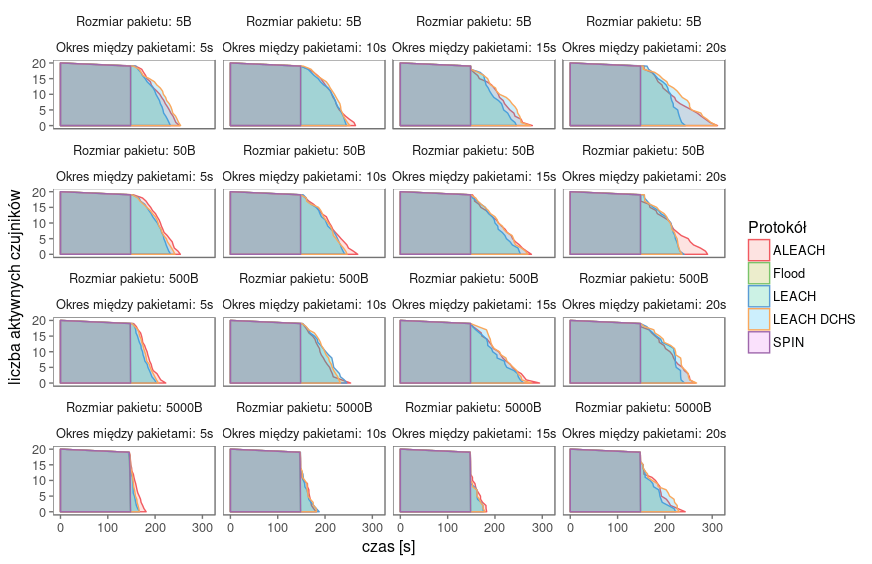
\includegraphics[width=308mm,height=229mm,page=1]{\ImgPath/charts/alive_nodes_normal_20sensors.png}}\endgraf
    \vspace{2ex}%
    \captionof{figure}{Aktywne węzły - 20 czujników, rozkład normalny}}}\kern-.5\pdfpagewidth
     \par
     \vspace*{-5cm}
\clearpage
\thispagestyle{empty}
    \vspace*{-2cm}
    \noindent\parbox{\textwidth}{%
    \noindent\rlap{\includegraphics[width=308mm,height=229mm,page=2]{\ImgPath/charts/stored_energy_normal_20sensors.png}}\endgraf
    \vspace{2ex}%
    \captionof{figure}{Energia sieci - 20 czujników, rozkład normalny}}
     \par
     \vspace*{-5cm}
\clearpage
}

Poniższe wykresy przedstawiają liczbę aktywnych węzłów sieci w czasie oraz w zależności od rozmiaru pakietu i odstępie czasu pomiędzy kolejnymi pakietami. Sieć składała się z dwustu węzłów, które rozmieszczone zostały zgodnie z rozkładem normalnym. Różnice pomiędzy wariantami protokołu LEACH są mniej wyraźne niż w przypadku sieci składającej się z dwudziestu węzłów. Najwrażliwszym na zmiany parametrów symulacji protokołem okazał się LEACH DCHS. Sieć go używająca działa wyraźnie krócej od pozostałych wariantów krótszych okresów pomiędzy pakietami oraz nieznacznie dłużej dla dłuższych okresów pomiędzy pakietami. Czas działania sieci dla protokołów Flood i SPIN podobnie jak w poprzednio pozostaje niezmienny, niezależnie od dobranych parametów wykresu.

\clearpage
\thispagestyle{empty}

{\pdfpagewidth=2\pdfpagewidth
    \vspace*{-2cm}
    \noindent\kern.5\pdfpagewidth\rlap{\parbox{\textwidth}{%
    \noindent\kern.25\pdfpagewidth
        \llap{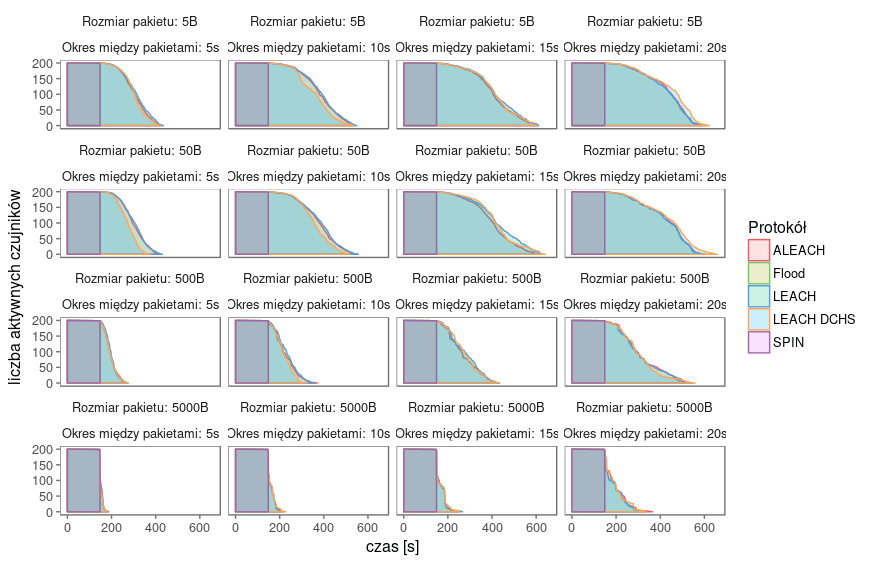
\includegraphics[width=308mm,height=229mm,page=1]{\ImgPath/charts/alive_nodes_normal_200sensors.png}}\endgraf
    \vspace{2ex}%
    \captionof{figure}{Aktywne węzły - 200 czujników, rozkład normalny}}}\kern-.5\pdfpagewidth
     \par
     \vspace*{-5cm}
\clearpage
\thispagestyle{empty}
    \vspace*{-2cm}
    \noindent\parbox{\textwidth}{%
    \noindent\rlap{\includegraphics[width=308mm,height=229mm,page=2]{\ImgPath/charts/stored_energy_normal_200sensors.png}}\endgraf
    \vspace{2ex}%
    \captionof{figure}{Energia sieci - 200 czujników, rozkład normalny}}
     \par
     \vspace*{-5cm}
\clearpage
}

Poniższe wykresy przedstawiają liczbę aktywnych węzłów sieci w czasie oraz w zależności od rozmiaru pakietu i odstępie czasu pomiędzy kolejnymi pakietami. Sieć składała się z dwudziestu węzłów, które rozmieszczone zostały zgodnie z rozkładem jednorodnym.
Najdłuższy czas działania sieci został osiągnięty przez protokół ALEACH. Jest to najbardziej widoczne przy dłuższych odstępach pomiędzy kolejnymi pakietami z danymi.
Tak samo, jak w poprzednio opisanych wynikach symulacji, zwiększenie rozmiaru danych oraz skrócenie czasu pomiędzy pakietami wpływa negatywnie na długość działania sieci oraz powoduje zacieranie się na tym polu różnic pomiędzy różnymi protokołami.


\clearpage
\thispagestyle{empty}

{\pdfpagewidth=2\pdfpagewidth
    \vspace*{-2cm}
    \noindent\kern.5\pdfpagewidth\rlap{\parbox{\textwidth}{%
    \noindent\kern.25\pdfpagewidth
        \llap{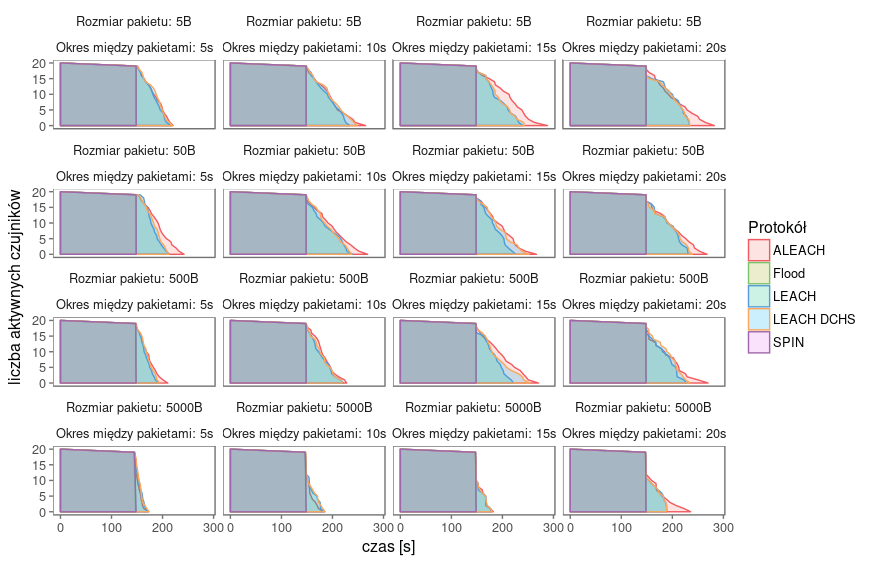
\includegraphics[width=308mm,height=229mm,page=1]{\ImgPath/charts/alive_nodes_uniform_20sensors.png}}\endgraf
    \vspace{2ex}%
    \captionof{figure}{Aktywne węzły - 20 czujników, rozkład jednorodny}}}\kern-.5\pdfpagewidth
     \par
     \vspace*{-5cm}
\clearpage
\thispagestyle{empty}
    \vspace*{-2cm}
    \noindent\parbox{\textwidth}{%
    \noindent\rlap{\includegraphics[width=308mm,height=229mm,page=2]{\ImgPath/charts/stored_energy_uniform_20sensors.png}}\endgraf
    \vspace{2ex}%
    \captionof{figure}{Energia sieci - 20 czujników, rozkład jednorodny}}
     \par
     \vspace*{-5cm}
\clearpage
}

\clearpage
\thispagestyle{empty}

{\pdfpagewidth=2\pdfpagewidth
    \vspace*{-2cm}
    \noindent\kern.5\pdfpagewidth\rlap{\parbox{\textwidth}{%
    \noindent\kern.25\pdfpagewidth
        \llap{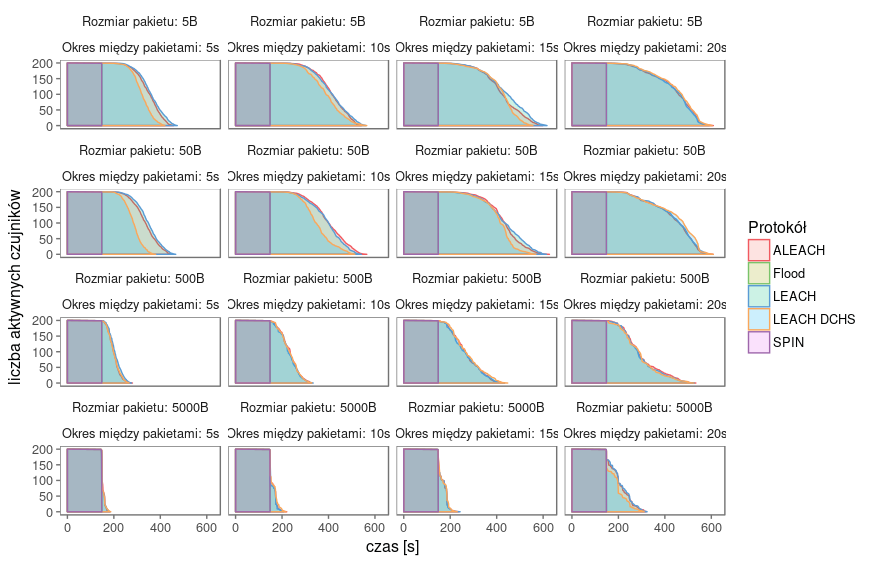
\includegraphics[width=308mm,height=229mm,page=1]{\ImgPath/charts/alive_nodes_uniform_200sensors.png}}\endgraf
    \vspace{2ex}%
    \captionof{figure}{Aktywne węzły - 200 czujników, rozkład jednorodny}}}\kern-.5\pdfpagewidth
     \par
     \vspace*{-5cm}
\clearpage
\thispagestyle{empty}
    \vspace*{-2cm}
    \noindent\parbox{\textwidth}{%
    \noindent\rlap{\includegraphics[width=308mm,height=229mm,page=2]{\ImgPath/charts/stored_energy_uniform_200sensors.png}}\endgraf
    \vspace{2ex}%
    \captionof{figure}{Energia sieci - 200 czujników, rozkład jednorodny}}
     \par
     \vspace*{-5cm}
\clearpage
}
